\documentclass{beamer}

\usepackage[ngerman]{babel}
\usepackage[utf8]{inputenc}
\usepackage[T1]{fontenc}
\usepackage{lmodern}
\usepackage{pdfpages}

\usetheme{Boadilla}  %% Themenwahl
\usecolortheme{whale}


%% Variables. You may want to change them. 
\title{Campusrallye}
\subtitle{}
\author{}
\date{\today}

\setbeamertemplate{headline}
{
  \leavevmode%
  \hbox{%
  \begin{beamercolorbox}[wd=\paperwidth,ht=8.25ex,dp=1.5ex]{palette secondary}
    \raggedright
    \hspace*{2em}%
    
\includegraphics[width=15mm]{media/fachschaft.png} 
    \hspace{100pt}
\includegraphics[width=5mm]{media/fakultaet_mathe.png}
    \hspace{10pt}
\includegraphics[width=5mm]{media/fakultaet_physik.png}
    \hspace{10pt}
\includegraphics[width=5mm]{media/fakultaet_informatik.png}
    \hspace{100pt}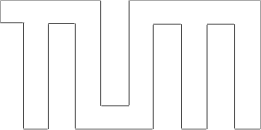
\includegraphics[width=10mm]{media/tum.png}
    \hspace*{2em}%
  \end{beamercolorbox}%
  }%
}


% If you want to get rid of the presentation controls in the bottom right corner, enable this setting
% \setbeamertemplate{navigation symbols}{} 

% This setting removes the footer but keeps the frame (=slide) number in the bottom right corner
% \setbeamertemplate{footline}[frame number]{}

% This setting removes the footer completely. It is going to override footer-related settings from above!
% \setbeamertemplate{footline}{}

%%%%%%%%%%%%%%%%%%%%%%%%%%%%%%%%%%%%%%%%%%%%%%%%%%%%%%%%%%%%%%%%%%%%%%%%%%%%%%%%%%%%%%%%%%%%%%%%%%%%%%%%%%%%%%%%%%%%%%%
% The content starts here
\begin{document}


	
	% First page
	\maketitle
	% Comment this out to remove the table of contents
	
	\begin{frame}
		\huge
		\center
		\frametitle{General}
		
		\begin{itemize}
			\item $\sim 60$  Tutors
			\item 21 Stations + Information desk + beverage sales 
			\item Each group should have >= 1 fully charged mobile phone!
		\end{itemize}
	\end{frame}
	
	
	
	\begin{frame}
		\huge
		
		\frametitle{Timetable}
		Saturday 12.10.2018\\
		
		\begin{itemize}
			\item 10:15: Meeting \normalsize in HS 1 \huge
			\item 11:00 - 14:00 + x: Rallye 
			\item approx. 15:00 : Award ceremony
		\end{itemize}
	\end{frame}
	
	
	
	
	\begin{frame}
		\huge
		\begin{center}
			Slack registration: \\
			\url{https://bit.ly/2p417os} \\ \ \\
		
		\end{center}
		\large
		\begin{itemize}
			\item Register with your real name!
			\item Install the Slack app on your phone!
			\item A list with all stations will be available on Thursday.
			\item You can also register directly as a group of two.
			\item Please choose your favourite stations til Friday evening.
			\item FCFS!
		\end{itemize}
		
	\end{frame}
	
	\begin{frame}
		\huge
		\begin{center}
			Slack registration: \\
			\url{https://bit.ly/2p417os} \\ \ \\
	
	
			Questions?		
		\end{center}
		\large
		

		
		
	\end{frame}
	%Diagramm über den Fakt, dass Übung sehr wichtig ist?!
	
	% Sections are like chapters and used to structure the presentation 

\end{document}
